\documentclass[10pt,a4paper]{article}
\usepackage{amsmath}
\usepackage{amsfonts}
\usepackage{amssymb}
\usepackage{graphicx}
\usepackage[frenchb]{babel}
\usepackage[utf8x]{inputenc}
\graphicspath{{images/}}
\usepackage{parskip}
\usepackage{fancyhdr}
\usepackage{vmargin}
\usepackage{caption}
\usepackage{subcaption}
\usepackage{hyperref}
\setmarginsrb{3 cm}{2.5 cm}{3 cm}{2.5 cm}{1 cm}{1.5 cm}{1 cm}{1.5 cm}

\title{Travaux pratiques avec Weka}                             % Title
\author{Maxime De Wolf}                               % Author
\date{\today}                                           % Date

\makeatletter
\let\thetitle\@title
\let\theauthor\@author
\let\thedate\@date
\makeatother

\pagestyle{fancy}
\fancyhf{}
\rhead{\theauthor}
\lhead{\thetitle}
\cfoot{\thepage}

\begin{document}
   	
   	%%%%%%%%%%%%%%%%%%%%%%%%%%%%%%%%%%%%%%%%%%%%%%%%%%%%%%%%%%%%%%%%%%%%%%%%%%%%%%%%%%%%%%%%%
   	
   	\begin{titlepage}
   		\centering
   		\vspace*{0.5 cm}
   		
\includegraphics[scale = 0.75]{UMONS}\\[1.0 cm]   % University Logo
   		\textsc{\LARGE Université de Mons}\\[2.0 cm]   % University Name
   		\textsc{\large Datawarehousing and datamining}\\[0.5 cm]               % Course Name
   		\rule{\linewidth}{0.2 mm} \\[0.4 cm]
   		{ \huge \bfseries \thetitle}\\
   		\rule{\linewidth}{0.2 mm} \\[1.5 cm]
   		
   		\begin{minipage}{0.4\textwidth}
   			\begin{flushleft} \large
   				\emph{Auteur:}\\
   				\theauthor
   			\end{flushleft}
   		\end{minipage}~
   		\begin{minipage}{0.4\textwidth}
   			\begin{flushright} \large
                                 % Your Student Number
   			\end{flushright}
   		\end{minipage}\\[2 cm]
   		
   		{\large \thedate}\\[2 cm]
   		
   		\vfill
   		
   	\end{titlepage}
   	
   	%%%%%%%%%%%%%%%%%%%%%%%%%%%%%%%%%%%%%%%%%%%%%%%%%%%%%%%%%%%%%%%%%%%%%%%%%%%%%%%%%%%%%%%%%
   	
   	\tableofcontents
   	\newpage
   	
   	%%%%%%%%%%%%%%%%%%%%%%%%%%%%%%%%%%%%%%%%%%%%%%%%%%%%%%%%%%%%%%%%%%%%%%%%%%%%%%%%%%%%%%%%%
   	
   	\section{Weka: Tutoriel}
   	
	   	\subsection{Questions 17.1.9 et 17.1.10}
		   	Ces questions portent sur l'arbre de décision crée à partir du fichier \textit{iris.arff}. Voici donc l'arbre de décision obtenu:
		   	
		   	\begin{figure}[h]
		   		\begin{center}
		   			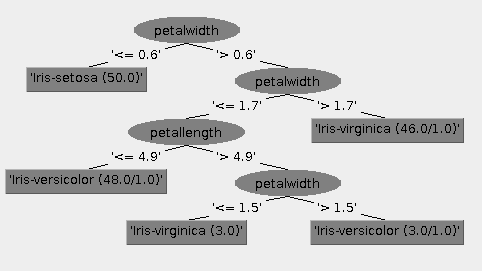
\includegraphics[width=0.3\linewidth]{IrisTree}
		   		\end{center}
		   		\caption{Arbre de décision du \textit{dataset iris.arff}}
		   		\label{fig-Iris-tree}
		   	\end{figure}
		   	
		   	\subsubsection*{Question 17.1.9}
			   	Cette question consiste à évaluer la qualité de cet arbre (Figure \ref{fig-Iris-tree}) grâce à différentes options de tests. Ici, on effectuera ces tests une première fois avec le \textit{dataset} complet et la $2^{e}$ fois avec la technique \textit{10-fold cross-validation}. Nous comparons ensuite les résultats obtenus sur base des 2 \textit{confusion matrix}:\\
	   			
	   			\begin{table}[h]
	   				\centering
					\begin{subtable}{0.4\textwidth}
						\centering
						\caption{\textit{Dataset} complet}
						\begin{tabular}{|c|c|c|l|}
							\hline
							a & b & c & \\ 
							\hline
							50 & 0 & 0 & a = Iris-setosa\\
							\hline
							0 & 49 & 1 & b = Iris-versicolor\\
							\hline
							0 & 2 & 48 & c = Iris-virginica\\
							\hline
						\end{tabular}
					\end{subtable}%
					\begin{subtable}{0.4\textwidth}
						\centering
						\caption{\textit{10-fold cross-validation}}
						\begin{tabular}{|c|c|c|l|}
							\hline
							a & b & c & \\ 
							\hline
							49 & 1 & 0 & a = Iris-setosa\\
							\hline
							0 & 47 & 3 & b = Iris-versicolor\\
							\hline
							0 & 2 & 48 & c = Iris-virginica\\
							\hline
						\end{tabular}
					\end{subtable}
					\caption{\textit{Confusion matrix} obtenues grâce à deux méthodes de test différentes}
	   			\end{table}
 
				 Nous remarquons que le test sur le \textit{dataset} complet classifie correctement $98\%$ des instances tandis que ce chiffre descend à $96\%$ avec le test \textit{10-fold cross-validation}. Tester le modèle avec le \textit{dataset} complet est une mauvaise idée car il donne une estimation optimiste de la qualité du modèle. En revanche, \textit{10-fold cross-validation} permet de se faire une bonne idée de la généralisation du modèle et offre donc une meilleure mesure de qualité.
				 
			\subsubsection*{Question 17.1.10}
			
				En observant la localisation de ces erreurs, nous remarquons que certaines instances de classe \textit{Iris-Verginica} ont des valeurs d'attributs équivalentes à celles d'instance de classe \textit{Iris-Versicolor}. Le modèle n'a donc aucune chance de les différencier si nous voulons éviter l'\textit{overfitting}. D'autre part, nous remarquons que l'instance de classe \textit{Iris-Setosa} qui a été mal identifier aurait dû être correctement classé selon l'arbre de décision final obtenu. 
		
		\subsection{Questions 17.2.4 à 17.2.11}
		
			\subsubsection*{Question 17.2.4}
				Le but de cette question est d'étudier la précision du classificateur \textit{5-nearest neighbor} en fonction des attributs utilisés lors de cette classification. Ici, nous exécutons cette algorithme sur le \textit{dataset glass.arff} et nous le test grâce à la technique \textit{10-fold cross-validation}. Les résultats ainsi obtenus sont résumés dans la table suivante:
				
				\begin{table}[h]
					\centering
					\caption{Précision obtenue en utilisant \textit{IBk} pour différents sous-ensemble d'attributs}
					\begin{tabular}{|c|c|c|}
						\hline
						Nombre d'attributs & Attribut retiré & Précision de la classification\\
						\hline
						9 & $\emptyset$ & 67.757 \\
						\hline
						8 & Si & 71.4953 \\
						\hline
						7 & Fe & 73.3645 \\
						\hline
						6 & Al & 73.3645 \\
						\hline
						5 & Na & 74.2991 \\
						\hline
						4 & Ba & 74.7664 \\
						\hline
						3 & K & 72.4299 \\
						\hline
						2 & Ca & 71.9626 \\
						\hline
						1 & Mg & 52.8037 \\
						\hline
						0 & RI & 35.514\\
						\hline
					\end{tabular}
				\end{table}
				
				Grâce à ce tableau, nous remarquons donc que la précision de \textit{IBk} sur le \textit{dataset} complet est de $67.757\%$ alors que nous obtenons une précision de $74.7664\%$ une fois que nous retirons les attributs \textit{Si, Fe, Al, Na, Ba} du \textit{dataset}. Ce qui nous donne un gain d'environ $7\%$ de précision.
			
			\subsubsection*{Question 17.2.5}
			
				Cette question demande de critiquer la pertinence de la précision maximum obtenue dans la question précédente. Ou, en d'autres mots, cette estimation est-elle biaisée ou non ?
				Etant donné que le test du modèle est effectué sur le \textit{dataset} d'entraînement, cette estimation est effectivement biaisée.
				
			\newpage
				
			\subsubsection*{Question 17.2.6}
				Cette question nous demande de constater l'effet du bruit sur un modèle construit grâce à \textit{IBk}. Pour ce faire, nous allons faire varier le pourcentage de bruits ainsi que la taille du voisinage dans les paramètres d'\textit{IBk}. Ainsi, une estimation de la précision sera calculé avec \textit{10-fold cross-validation}. Il est important de noter que ce test se fera sans les ajouts de bruits. Il n'y a donc présence de bruit que lors de la phase d'entraînement mais pas lors de la phase de test. La table suivante résume les résultat obtenus: 
			
				\begin{table}[h]
					\centering
					\caption{Effet du bruit sur la précision d'\textit{IBk}, en fonction de différentes tailles de voisinage}
					\label{tab-IBk-noise}
					\begin{tabular}{|c|c|c|c|}
						\hline
						Pourcentage de bruit & k = 1  & k = 3  & k = 5  \\
						\hline
						$0\%$ & $70.6\%$ & $72.0\%$ & $67.8\%$ \\
						\hline
						$10\%$ & $62.6\%$ & $69.6\%$ & $64.5\%$ \\
						\hline
						$20\%$ & $50.5\%$ & $63.1\%$ & $61.7\%$ \\
						\hline
						$30\%$ & $47.2\%$ & $58.4\%$ & $59.8\%$ \\
						\hline
						$40\%$ & $41.1\%$ & $54.7\%$ & $55.1\%$  \\
						\hline
						$50\%$ & $33.2\%$ & $44.4\%$ & $45.3\%$ \\
						\hline 
						$60\%$ & $27.1\%$ & $35.5\%$ & $35.5\%$ \\
						\hline 
						$70\%$ & $20.1\%$ & $28.5\%$ & $29.0\%$ \\
						\hline 
						$80\%$ & $14.0\%$ & $21.0\%$ & $21.0\%$ \\
						\hline 
						$90\%$ & $7.9\%$ & $13.6\%$ & $9.3\%$ \\
						\hline 
						$100\%$ & $4.7\%$ & $7.9\%$ & $7.5\%$ \\
						\hline 
					\end{tabular}
				\end{table}
				
			\subsubsection*{Question 17.2.7}
			
				Cette question nous demande de critiquer les résultats obtenues lors de la question précédente. Plus particulièrement, on nous demande l'effet qu'a une augmentation du bruit au niveau de la classe. La Table \ref{tab-IBk-noise} nous permet de constater que cette augmentation réduit la précision du classificateur \textit{k-nearest neighbor} et ce peu importe la valeur du k.
				
			\subsection*{Question 17.2.8}
				
				Cette question s'intéresse plutôt aux effets qu'a la modification de la valeur de k pour le classificateur \textit{k-nearest neighbor}. Dans la Table \ref{tab-IBk-noise} nous remarquons qu'augmenter la valeur de k rend le modèle obtenu plus robuste au bruit.\\
				
				En effet, nous remarquons que bien qu'il n'y ait pas de différence significative entre les modèles obtenus pour k = 3 et k = 5, ils sont plus résistants au bruit que ceux obtenus pour k = 1.
				
			\newpage
				
			\subsection*{Question 17.2.9}
				Pour cette question, nous devons comparer les classificateurs \textit{IBk} et \textit{J48} en fonction du pourcentage de l'ensemble d'apprentissage utilisé. Ces résultats sont encodés dans la table suivante:
			
				\begin{table}[h]
					\centering
					\caption{Variation de la précision du modèle en fonction de la taille de l'ensemble d'apprentissage pour \textit{IBk} et \textit{J48}}
					\label{tab-IBk-J48}
					\begin{tabular}{|c|c|c|}
						\hline
						Pourcentage de l'ensemble d'apprentissage & \textit{IBk} & \textit{J48}\\
						\hline
						$10\%$ & $52.8\%$ & $45.3\%$ \\
						\hline
						$20\%$ & $63.6\%$ & $53.3\%$ \\
						\hline
						$30\%$ & $60.3\%$ & $59.3\%$ \\
						\hline
						$40\%$ & $63.6\%$ & $65.0\%$ \\
						\hline
						$50\%$ & $62.6\%$ & $63.1\%$ \\
						\hline
						$60\%$ & $64.5\%$ & $69.2\%$ \\
						\hline
						$70\%$ & $65.9\%$ & $67.8\%$ \\
						\hline
						$80\%$ & $67.8\%$ & $70.1\%$ \\
						\hline
						$90\%$ & $67.3\%$ & $69.6\%$ \\
						\hline
						$100\%$ & $66.8\%$ & $68.2\%$ \\
						\hline
					\end{tabular}
				\end{table}
   	
   	\section{CoIL Challenge 2000}
   	
          	
\end{document}